%; whizzy chapter
% -initex iniptex -latex platex -format platex -bibtex jbibtex -fmt fmt
% 以上 whizzytex を使用する場合の設定。

%     Kansai Debian Meeting resources
%     Copyright (C) 2007 Takaya Yamashita
%     Thank you for Tokyo Debian Meeting resources

%     This program is free software; you can redistribute it and/or modify
%     it under the terms of the GNU General Public License as published by
%     the Free Software Foundation; either version 2 of the License, or
%     (at your option) any later version.

%     This program is distributed in the hope that it will be useful,
%     but WITHOUT ANY WARRANTY; without even the implied warranty of
%     MERCHANTABILITY or FITNESS FOR A PARTICULAR PURPOSE.  See the
%     GNU General Public License for more details.

%     You should have received a copy of the GNU General Public License
%     along with this program; if not, write to the Free Software
%     Foundation, Inc., 51 Franklin St, Fifth Floor, Boston, MA  02110-1301 USA

%  preview (shell-command (concat "evince " (replace-regexp-in-string "tex$" "pdf"(buffer-file-name)) "&"))
% 画像ファイルを処理するためにはebbを利用してboundingboxを作成。
%(shell-command "cd image200708; ebb *.png")

%%ここからヘッダ開始。

\documentclass[mingoth,a4paper]{jsarticle}
\usepackage{kansaimonthlyreport}
\usepackage[dvips]{xy}

% 日付を定義する、毎月変わります。
\newcommand{\debmtgyear}{2012}
\newcommand{\debmtgdate}{22}
\newcommand{\debmtgmonth}{7}
\newcommand{\debmtgnumber}{61}

\begin{document}

\begin{titlepage}

% 毎月変更する部分、本文の末尾も修正することをわすれずに

 第\debmtgnumber{}回 関西 Debian 勉強会資料

\vspace{2cm}

\begin{center}
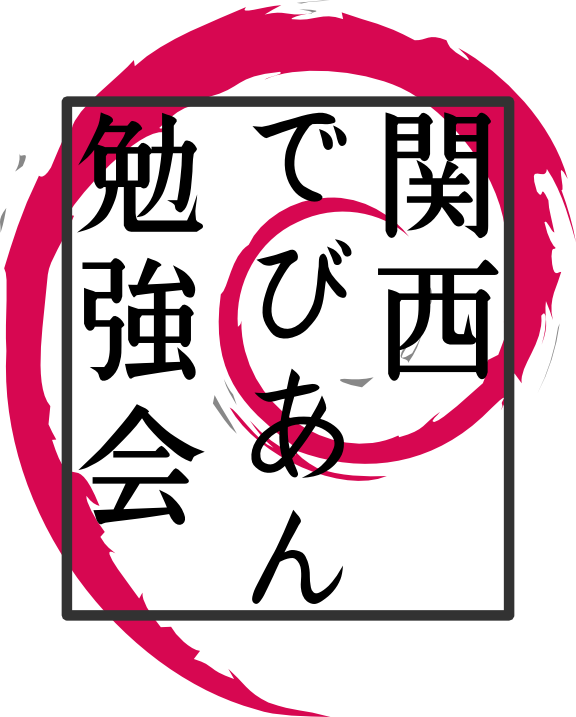
\includegraphics{image200802/kansaidebianlogo.png}
\end{center}

\begin{flushright}
\hfill{}関西 Debian 勉強会担当者 佐々木・倉敷・のがた・かわだ \\
\hfill{}\debmtgyear{}年\debmtgmonth{}月\debmtgdate{}日
\end{flushright}

\thispagestyle{empty}
\end{titlepage}

\dancersection{Introduction}{Debian JP}

 関西Debian勉強会はDebian GNU/Linuxのさまざまなトピック
 (新しいパッケージ、Debian特有の機能の仕組、Debian界隈で起こった出来事、
 などなど)について話し合う会です。

 目的として次の三つを考えています。
 \begin{itemize}
  \item MLや掲示板ではなく、直接顔を合わせる事での情報交換の促進
  \item 定期的に集まれる場所
  \item 資料の作成
 \end{itemize}

 それでは、楽しい一時をお楽しみ下さい。

\newpage

\begin{minipage}[b]{0.2\hsize}
 {\rotatebox{90}{\fontsize{80}{80}
{\gt 関西 Debian 勉強会}}}
\end{minipage}
\begin{minipage}[b]{0.8\hsize}
\hrule
\vspace{2mm}
\hrule
\setcounter{tocdepth}{1}
\tableofcontents
\vspace{2mm}
\hrule
\end{minipage}

\dancersection{最近のDebian関係のイベント報告}{Debian JP}

\subsection{大統一 Debian 勉強会}
来る 6 月 23 日に東京エリア Debian 勉強会と合同の勉強会として大統一 Debian 勉強会
が開催されました。

当日のセッションの内容についてはこの後の「大統一 Debian 勉強会の報告」で。


\subsection{第 90 回東京エリア Debian 勉強会}
90 回目の東京エリア Debian 勉強会は 7 月 21 日に開催されました。

MacBook Air に Debian と Debconf12 について語るの二本立てでした。

2011 年モデルの MacBook Air に Debianをインストールしてみようと思われている方は
参考にされてみてはいかがでしょうか。

Debconf12 のセッション一覧\footnote{\url{http://penta.debconf.org/dc12_schedule/events.en.html}}
とビデオ\footnote{\url{http://mirrors.mithril-linux.org/debconf12/}}
が公開されています。興味のあるセッションがあれば見てみてください。

\clearpage

\clearpage

%debianmeetingresume201010.tex
%-------------------------------------------------------------------------------
\dancersection{大統一 Debian 勉強会 2012 参加報告}{DebianJP}
%-------------------------------------------------------------------------------

\label{sec:gumreportsummary}
\index{GUM2012}
\index{GUM}

\subsection{大統一 Debian 勉強会とは}

Debian JP では、東京と関西の 2 ヶ所を中心に、毎月 Debian 勉強会を開催しています。今回、それらをまとめて、大統一 Debian 勉強会としてイベントの規模を拡大して実施しました。

通常顔をあわせることのないメンバーたちが日本各地から一同に介し友好を深め、技術的な議論を戦わせます。

\subsubsection{大統一 Debian 勉強会 2012}

第一回目の大統一 Debian 勉強会は、2012年6月23日に、京都の京都大学で開催されました。毎月の勉強会でお馴染みの人たちはもちろん、日本各地から参加者があり、最終的には 100 名弱のイベントとなりました。

\subsubsection{会場}

京都大学の数学教室をお借りして、カンファレンス用に 2部屋、ハックラボとして 1部屋が用意されました。
休日の大学ということもあって、構内は比較的落ちついており、勉強会の開催も違和感なくとけこんでいたように思います。

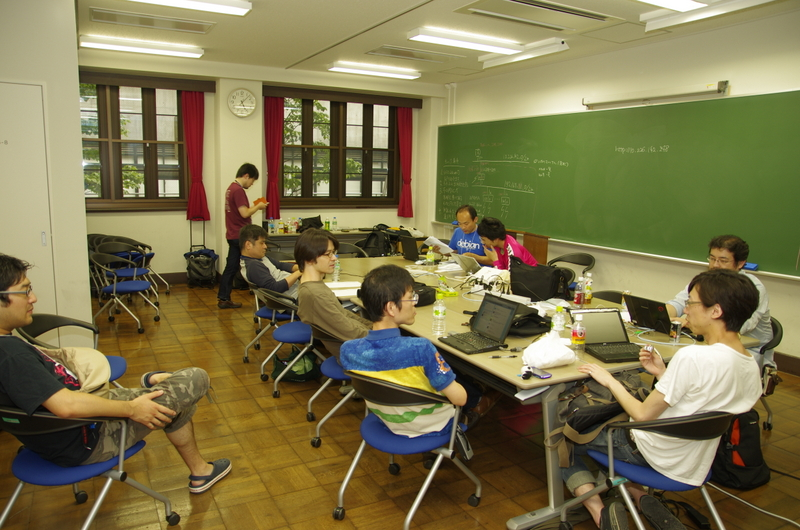
\includegraphics[width=0.8\hsize]{image201206/gum2012-hacklab.jpg}

今回は、参加者向けのネットワークとして、無線 AP を用意して京都大学の Proxy 経由で外部に出ていくようにしていました。無線の調子は悪くなかったようですが、Proxy の設定でつまづく人はそれなりにいたようです。
また、WiMAX ルータを使って Ustream 中継をする予定にしていましたが、やはりというかセッション中は自前の Wifi ルータを使う参加者が多かったようで、接続が全く安定しませんでした。

\subsection{スケジュールとイベント}

開催期間は 1 日間のみで、Debconf のような催事はおりこまれていません。Debian 勉強会としては初の試みになりますが、2 トラックでのセッション運営を行い、合計 13 (加えて LT 5件) のセッションが行われました。

セッションの一環として、おなじみのキーサインパーティも開催され、28 名の参加者がありました。また、パーティには参加せず、個人的にキーサインを行う人もいたようです。

\subsection{セッション}

トラックを 2 つ設けたとはいっても、特にカテゴリの設定などはしませんでした。セッション内容も Debian 固有の開発話から Linux 全般に通じるネタ、組み込みやデバイス関連の Tips から便利なアプリケーションの紹介まで、千差万別でした。

セッションの内容は、下記の通りです。\footnote{http://gum.debian.or.jp/ のタイムテーブルに、当日の発表資料と titanpad によるディスカッションの記録が保存されています}

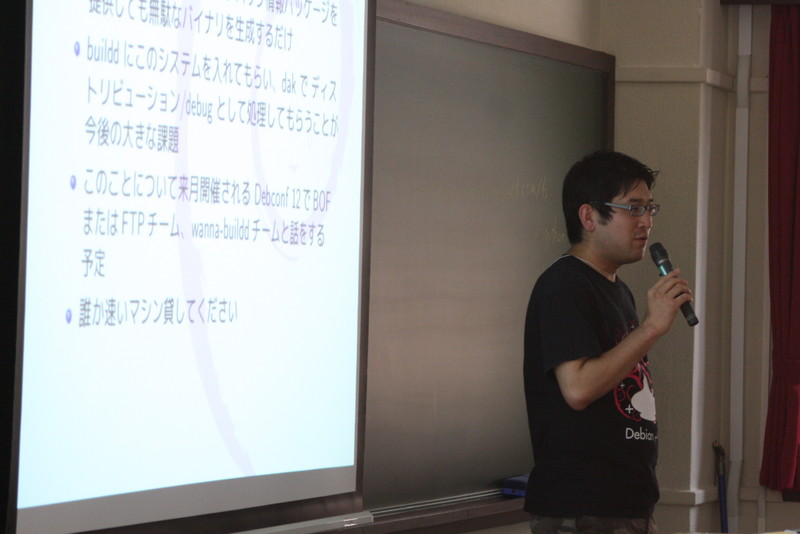
\includegraphics[width=8cm]{image201206/gum2012-session2.jpg}
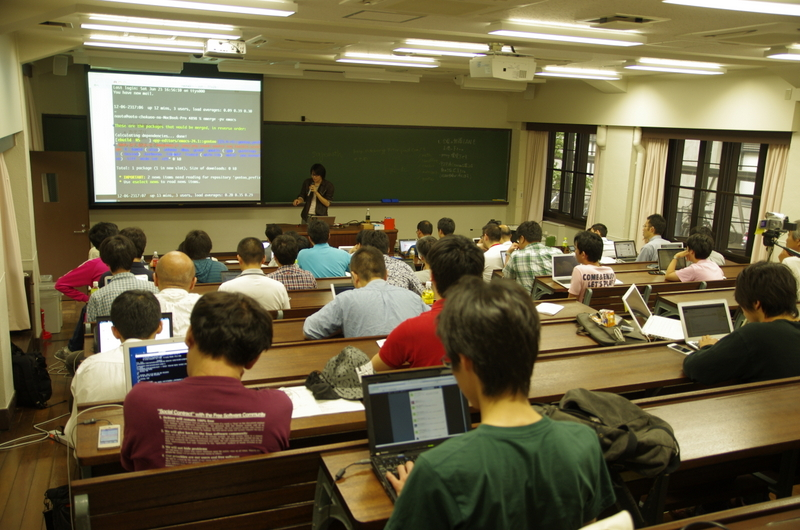
\includegraphics[width=8cm]{image201206/gum2012-session1.jpg}

\subsubsection{TeXLive 2011(2012/dev) in Debian / 発表者 佐々木洋平}

pTeX がドロップされるなど、大きな変更が予定されている Wheezy 向けの \TeX 環境の現状紹介と、日本語処理面での導入、設定方法の説明がされました。

\subsubsection{Linux-PAM の設定について / 発表者 西山和広}

pam-auth-update など、独自のユーティリティに触れたりしつつも、PAM の構成や設定について、基本的なところから解説されていました。

\subsubsection{数学ソフトウェア使ってますか? / 発表者 濱田龍義}

最近 MathLibre と改名した、数学ソフトウェアに特化したライブディストリビューションと、収録されている数学ソフトウェアを紹介するセッションでした。

\subsubsection{ipython notebook とその周辺 / 発表者 本庄 弘典}

最近 Debian にインストールされた ipython notebookとその周辺ツールである ipython qtconsoleおよびipython nodebookの導入方法、使い方について説明
されました。

\subsubsection{Debian と LibreOffice / 発表者 あわしろ いくや}

OpenOffice から LibreOffice への変遷を軸に、Debian でのパッケージング状況や翻訳活動の紹介などが説明されていました。

\subsubsection{debug.debian.net / 発表者 岩松 信洋}

現在、Debian のバイナリパッケージは、コンパイル時にデバッグ情報が削除されています。デバッグなどの際に必要になるこのデータを提供しようというプロジェクトについての検討報告でした。休眠していた同様のプロジェクトを復活させる方向で動いているそうです。

\subsubsection{Rabbit: 時間内に終われるプレゼンツール / 発表者 須藤 功平}

どのようにプレゼンを行うのか、という観点も含めて Rabbit というプレゼンツールの背景にある設計思想を作者さん自らが解説する、というセッションでした。

\subsubsection{U-Bootについてあれこれ / 発表者 野島 貴英}

組み込み分野でよく利用されているブートローダである U-Boot の紹介と、Barnes \& Noble社Nook Color 向けに移植した例を紹介しました。

\subsubsection{Debian Multiarch Support / なかお けいすけ}

次期Debianのリリースゴールの一つに挙げられている Multiarch Support について仕組みと
現状について説明されました。

\subsubsection{家庭内LANを高速に! InfiniBand on Debian}

eBay で安価に機材を入手する方法から、Debian 上での利用方法、また高速な通信についての悦びまで、幅広く説明されていました。

\subsubsection{Gentoo/Prefix on Debian}

Gentoo Linux には、どんな OS にも Gentoo の皮をかぶせてしまう Prefix という仕掛け (平たく言うと chrooted gentoo) があります。
それを一歩進めて、Debian パッケージとの連携を深める試みについてのセッションでした。

\subsubsection{Debian でもマルチタッチ!}

Ubuntu が独自実装している関連パッケージを Debian にバックポートする方法の説明や、タッチパッドに指を何本も認識させるデモが行われていました。


\subsection{Lightning talk}
閉会直前に用意していた LT の枠も、事前の発表募集に反応が薄かったわりには当日の発表希望が複数あったため、なんとか無事に終えることができました。
LT のほとんどが Debian Developer によるものでしたが、これはさすがというべきか何というべきか....。

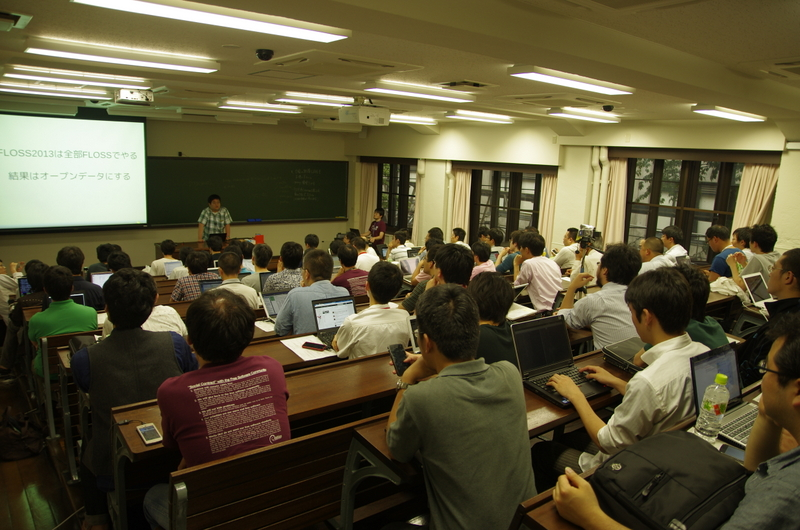
\includegraphics[width=8cm]{image201206/gum2012-lt.jpg}
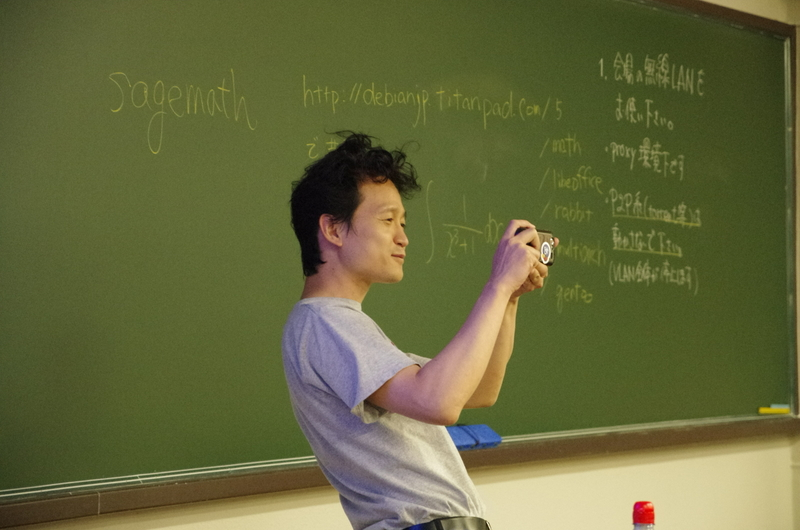
\includegraphics[width=8cm]{image201206/gum2012-closing.jpg}

\subsection{懇親会}

閉会後、会場近くの居酒屋で懇親会を行いました。総勢 60 名弱の参加者があり、普段の勉強会とは一味違うもりあがりを見せていました。

\subsection{次回の大統一 Debian 勉強会}

今のところ、次回の予定はたっていません。今回を盛況のうちに終えることができたので、何らかの企画はなされるはずです。乞うご期待。



\dancersection{事前課題}{Debian JP}

今回は以下の課題を出題しました.
\begin{screen}
  \begin{enumerate}
  \item Linux(Unix?)における login 時のユーザ認証の流れについて調べて(復習して)おいて下さい。\\
    大統一 Debian 勉強会の西山さんの発表資料などを参考にしてください。

  \item man 5 ldif などを参考に ldif ファイル形式のフォーマットを説明してください。\\
    何か一つでかまいませんのでディレクティブ、エントリの扱い方などの具体例をあげて説明してください。\\
    ldif.5.gz は ldap-utils パッケージで提供されています。

  \end{enumerate}
\end{screen}

参加者の皆さんの解答は以下の通りです。

\begin{prework}{ のがたじゅん }
  (無回答)
\end{prework}

\begin{prework}{ 佐々木洋平 }
とりあえず発表で。
\end{prework}

\begin{prework}{ 川江 }
  (無回答)
\end{prework}

\begin{prework}{ かわだてつたろう }
  \begin{enumerate}
  \item 西山さんの資料を読みました。
  \item フォーマットは次の形式。base64 エンコードと URL の場合が異なる。
    \begin{commandline}
      dn: <distinguished name>
      <attrdesc>: <attrvalue>
      <attrdesc>:: <base64-encoded-value>
      <attrdesc>:< <URL>
    \end{commandline}
    エントリを変更するには changetype ディレクティブ、属性には modify, add, delete, modrdn を指定する。modrdn は識別名を変更するのに使用する。
    \begin{commandline}
      changetype: <[modify|add|delete|modrdn]>
    \end{commandline}
  \end{enumerate}
\end{prework}

\begin{prework}{ 岡野孝悌 }
申し訳ありませんが間に合いませんでした。
(ldif(5)とRFC 2849は読みましたがそもそもLDAPがさっぱりわからん)
\end{prework}

\begin{prework}{ 甲斐正三 }
回答無しで済みません。
極力勉強会までにみておきます。
\end{prework}

\begin{prework}{ lurdan }
  \begin{enumerate}
  \item login/ssh/xdm → NSS → PAM → (module いろいろ)
  \item
    \begin{commandline}
      cn=lurdan,ou=People,dc=debian,dc=or,dc=jp (ノード名)
      changetype: add (どういう変更をするのか)
      objectClass: posixAccount (エントリ全体の意味付け)
      uid: 1000
      homeDirectory: /home/lurdan
      shell: /usr/bin/zsh
      ...
      ...
    \end{commandline}
  \end{enumerate}
\end{prework}

\begin{prework}{ 山城の国の住人 久保博 }
  \begin{enumerate}
  \item 西山さんの発表資料を読みました。
  \item ldif ディレクトリオブジェクトを記述するファイル形式です。テキスト
    形式の一種で、テキストエディタで編集できます。複数のエントリが並び、
    エントリ間は空行で区切られます。ldif のエントリは、ディレクトリオブジェ
    クトを表します。エントリの欄は 属性名と属性値をコロンで区切った行が並
    んだ形をしています。最初に現れる属性名 dn は、一意にそのオブジェクト
    を特定する、階層的な名前です。その以降、その他の属性の名前とその値が
    並びます。同じ属性名の行が複数現れても構いません。特別な属性とし
    て、objectClass があり、オブジェクトのスキーマを表します。一つのエン
    トリは、複数の objectClass を持てます。

    以下は、とある架空のサーバーのユーザーアカウントを表すエントリの例です。
    \begin{commandline}
      dn: uid=hiroshi,ou=Users,dc=kansai,dc=debian,dc=or,dc=jp
      objectClass: top
      objectClass: inetOrgPerson
      objectClass: posixAccount
      objectClass: shadowAccount
      objectClass: sambaSamAccount
      objectClass: inetLocalMailRecipient
      cn: Hiroshi Kubo
      uid: hiroshi
      uidNumber: 60001
      gidNumber: 60001
      homeDirectory: /home/hiroshi
      gecos: Hiroshi Kubo
      description: Hiroshi Kubo
      structuralObjectClass: inetOrgPerson
      entryUUID: 22012ece-8e45-102a-9c5d-fe1f8f03b311
      creatorsName: cn=manager,dc=kansai,dc=debian,dc=or,dc=jp
      createTimestamp: 20060612095407Z
      sambaLogonTime: 0
      sambaLogoffTime: 2147483647
      sambaKickoffTime: 2147483647
      displayName: Hiroshi Kubo
      sambaSID: S-1-5-21-4242558920-1755843709-XXXXXXXXX-XXXXX
      sambaLogonScript: hiroshi.cmd
      mailRoutingAddress: hiroshi.kubo@kansai.debian.or.jp
      sambaPrimaryGroupSID: S-1-5-21-4242558920-1755843709-119024134-1101
      sambaHomeDrive: H:
      mailLocalAddress: hiroshi
      mail: hiroshi.kubo@kansai.debian.or.jp
      sambaPasswordHistory: 0000000000000000000000000000000000000000000000000000000000000000
      sambaLMPassword: XXXXXXXXXXXXXXXXXXXXXXXXXXXXXXXX
      sambaAcctFlags: [U]
      sambaNTPassword: XXXXXXXXXXXXXXXXXXXXXXXXXXXXXXXX
      sambaPwdCanChange: 1200461017
      sambaPwdMustChange: 2147483647
      sambaPwdLastSet: 1200461017
      userPassword:: XXXXXXXXXXXXXXXXXXXXXXXXXXXXXXXXXXXXXXXXXXXXXXXXXXX=
      shadowLastChange: 14839
      sn: Kubo
      loginShell: /bin/bash
      entryCSN: 20120312100613.875600Z\#000000\#000\#000000
      modifiersName: cn=manager,dc=kansai,dc=debian,dc=or,dc=jp
      modifyTimestamp: 20120722000013Z
    \end{commandline}
  \end{enumerate}
\end{prework}
\begin{prework}{ daisuke\_oka@nanosoftware.biz }
(無回答)
\end{prework}

\begin{prework}{ kino }
  \begin{itemize}
  \item ldif ファイル形式のフォーマット
    \begin{commandline}
    dn: (distinguished name) と 
    attrdesc: attrvalue  からなる属性の組み合わせで一つのエントリーを記述。
    \end{commandline}
    objectClass: がよくわかってません。
    \begin{itemize}
    \item Attribute Type
    \end{itemize}
    \begin{commandline}
      CN Common Name
      L  Locality Name
      ST State Or Province Name
      O  Organization Name
      OU Organizational Unit Name
      C  Country Name
      STREET Street Address
      DC Domain Compornent
      UID User ID
    \end{commandline}
  \item どれを使ってよいのかよくわかってません。
    \begin{commandline}
      dn: uid=kino,ou=web,o=ANNAI,dc=an-nai,dc=jp
      uid: kino
      userPassword: hogehoge
      loginShell: /bin/bash
      homeDirectory: /home/kino
      objectClass: posixAccount
    \end{commandline}
  \end{itemize}
\end{prework}

\clearpage

\dancersection{Debian で作る LDAP サーバ}{佐々木 洋平}

\vspace{1em}%
先月は体調不良により穴をあけてしまい、大変すいませんでした。また、この場
を借りて急遽 X.500 の解説して下さった久保さんに御礼を。ありがとうございま
した。

\subsection{はじめに}

京都に来てから最初にやった業務は\texttt{Solaris8}と\texttt{NIS}の撲滅でし
た。特に複雑な要件は無かったのでOpenLDAPに移行して、ここ数年は順調に動作
して(いると思って)います。

$\cdots$で、気がついたら手元の仮想マシン群(各種Linuxディストリビューショ
ン、FreeBSD、Windows7など)の認証も、ホストOS(Debian)のOpenLDAPで行なうよ
うになっていました。ラップトップで常に\texttt{slapd}を上げているのもなん
かアレですが、気にしたら負けです。

とういわけで、ここでは「DebianでOpenLDAPサーバ(\texttt{slapd})を動かして、
色んなユーザ認証を一本化するまで」のお話をしてみたいと思います。
%
ちなみに、この企画を思いついた理由は「ネット上にある多くのドキュメントが
古い\texttt{slapd}について書かれていて、実際に運用しようとしたら色々とハ
マったから」だったんですが、先日倉敷さんに「Ubuntu Server Guide読んでねー
のかよ(ry」とバッサリ言われてしまいました。$\cdots$で読んでみたら、記事を
書く気力が $\cdots$。

気をとりなおして、先に進みます。

\subsection{LDAP:Lightweight Directory Access Protocol}

LDAP はディレクトリサービス(正確には X.500 モデルをサポートするディレクト
リサービス)に接続するために使用するためのプロトコルの一つです。ここでの
「ディレクトリ」はファイルを管理する階層構造ではなくて、「住所氏名録、人
名簿」の意味でのディレクトリです。X.500 データモデルはデータ構造(X.500)、
認証(X.509)、分散処理(X.518)、複製(X.525)といった標準規格と、これらにアク
セスするためのプロトコルである DAP: Directory Access Protocol があります。
この DAP を軽量化し、TCP/IP の上で実装したのが LDAP です。

\subsection{DIT: Directory Information Tree}

LDAPがアクセスするディレクトリデータは「住所録・名簿」であり、「人」や
「物」及びこれらに付随する情報(パスワードやメールアドレスなど)を管理する
ことに特化しています。これらの情報は頻繁に参照されることはあっても、更新
はさほど行なわれません。この点は MySQL などのリレーショナルデータベースと
異なる点です。

LDAP のアクセスするデータベースは「木構造」になっています。この木構造
を DIT と呼びます。DIT の各ノードは「エントリ」と呼ばれ、これらエントリに
は rdn: Relative Distinguished Name(相対識別名)が付いています。rdn をつな
げることで、エントリの dn:Distinguished Name(識別名)が一意に定まり、DIT
中で識別されます。ひとつのエントリには「属性名」と「属性値」がペアとなっ
て幾つか格納されています。属性名と属性値のテンプレートが objectClass です。
図(\ref{fig:DIT})に、DIT の例を示します。この例で
は、\texttt{localhost.localdomain}上で objectClass として \texttt{person} を用いて、
アカウント名とパスワードによる認証情報が格納されています。
\begin{figure}[h!]
  \begin{tabular}{cc}
    \begin{minipage}{0.38\linewidth}
      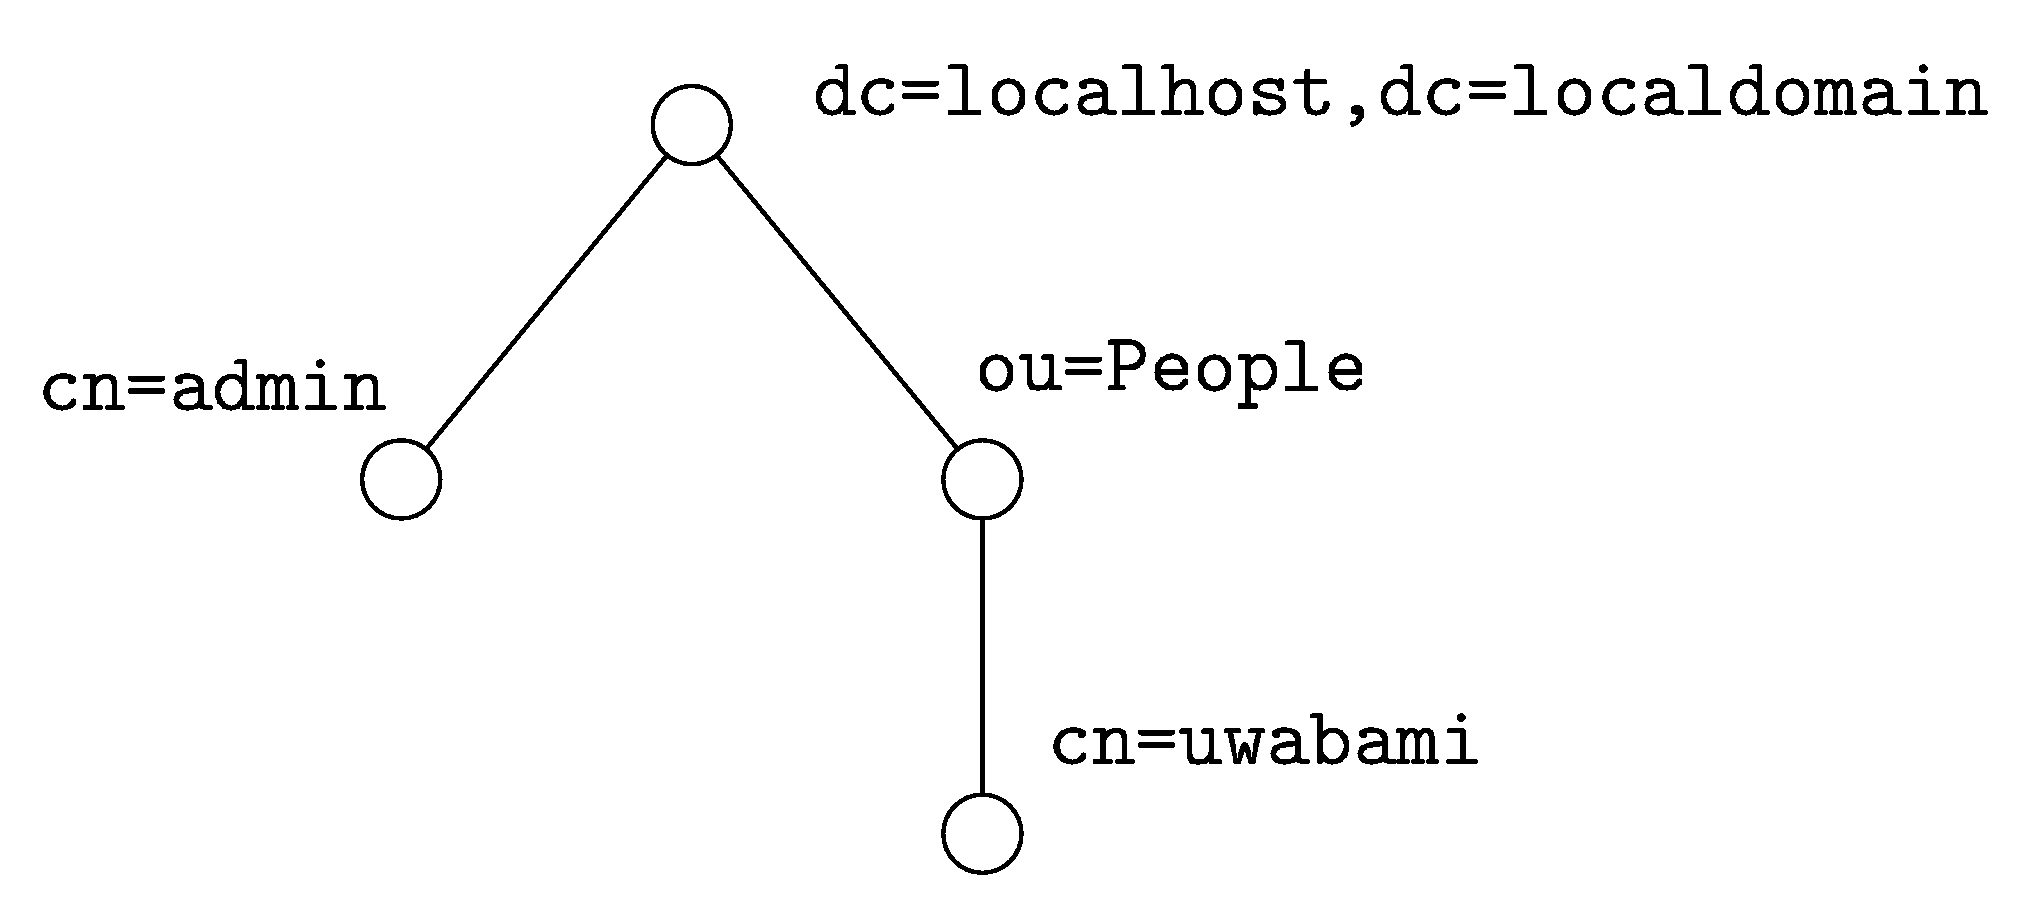
\includegraphics[width=.98\linewidth]{image201207/ldap-node-example.png}
    \end{minipage}
    \begin{minipage}{0.6\linewidth}
      \vspace{3em}
      \begin{screen}
        {\small
        \texttt{cn=uwabami,ou=People,dc=localhost,dc=localdomain}
        \begin{tabular}{ll}
          \texttt{objectClass}:
          & \texttt{person}                                 \\
          \texttt{cn}:
          & \texttt{Youhei SASAKI}                          \\
          \texttt{sn}:
          & \texttt{SASAKI}                                 \\
          \texttt{userPassword}:
          & \texttt{\{SSHA\}jP68h6yzJOlnRMda7IFI0LrTSe/lrFgO} \\
          $\cdots$ &\\
        \end{tabular}
        }
      \end{screen}
    \end{minipage}
  \end{tabular}
  \caption{DITの例。この場合
    の rootdn は \texttt{dc=localhost,dc=localdomain}となり、一番右下のエ
    ントリの dn は \texttt{cn=uwabami,ou=People,dc=localhost,dc=localdomain}と
    なる。}
  \label{fig:DIT}
\end{figure}

DIT中のエントリにどの様な情報を格納するのか、というスキーマ
は objectClass の集りであり、代表的な用途に用いられるスキーマは既に提供さ
れています。また、必要な情報を独自に定義して、新たに格納することも可能です。

\subsection{OpenLDAPの導入と初期設定}

LDAP サーバを導入して試してみます。Debianでは OpenLDAP サーバ
は \texttt{slapd} としてパッケージ化されていますので、これを導入します。
%
とりあえずラップトップの母艦と仮想マシン上の複数のクライアントを想定しますので
\begin{center}
  \texttt{rootdn: dc=vmhost,dc=localdomain}
\end{center}
で設定を始めてみます。

先ずは名前解決ができるようにしておきます。
自前で DNS を上げているのであれば問題無いのですが、
そうではない場合に備えて /etc/hosts あたりに
\begin{commandline}
  127.0.1.1     vmhost.localdomain vmhost
\end{commandline}
などと追記して
\texttt{dig}や\texttt{nslookup}で名前解決ができることを確認しておきます.
%
続いてインストールです。
\begin{commandline}
  $ sudo -s
  # apt-get install slapd ldap-utils
\end{commandline}
%$
debconf の dialog が出てくるので適宜答えると良いでしょう。
\begin{enumerate}
\item Omit OpenLDAP server configuration?
  → No
\item DNS domain name:
  → vmhost.localdomain
\item Organization name:
  → localdomain
\item Administrator password:
  → 適宜
\item Database backend to use: BDB でも HDB でもお好きな方を.
  HDB は subtree の rename をサポートしている。
\item Do you want to the database to be removed when slapd is purged?
  → Yes
\item Allow LDAPv2 protocol?
  → No
\end{enumerate}
この状態で、LDAP のデータベースには二つの DIT が存在します。
一つ目は管理用の DIT、二つ目はサービス用のデータを入れていく DIT です。
それぞれ以下で確認できます。
\begin{commandline}
$ sudo ldapsearch -Q -LLL -Y EXTERNAL -H ldapi:/// -b cn=config dn
dn: cn=config

dn: cn=module{0},cn=config

dn: cn=schema,cn=config

dn: cn={0}core,cn=schema,cn=config

dn: cn={1}cosine,cn=schema,cn=config

dn: cn={2}nis,cn=schema,cn=config

dn: cn={3}inetorgperson,cn=schema,cn=config

dn: olcBackend={0}hdb,cn=config

dn: olcDatabase={-1}frontend,cn=config

dn: olcDatabase={0}config,cn=config

dn: olcDatabase={1}hdb,cn=config

$ sudo ldapsearch -x -LLL -H ldap:/// -b dc=vmhost,dc=localdomain dn
dn: dc=vmhost,dc=localdomain

dn: cn=admin,dc=vmhost,dc=localdomain
\end{commandline}

では次に、ユーザ認証/管理ができるようにしてみます。
/etc/{passwd,shadow,groups} 相当のスキーマとして、
\begin{itemize}
\item \texttt{ou=People,dc=vmhost,dc=localdomain}というエントリ以下にユーザを格納
\item \texttt{ou=Groups,dc=vmhost,dc=localdomain}というエントリ以下にグループを格納
\item \texttt{cn=uwabami,ou=Groups,dc=vmhost,dc=localdomain}というグループを追加
\item \texttt{cn=uwabami,ou=People,dc=vmhost,dc=localdomain}というユーザを追加
\end{itemize}
する LDIF(LDAP Data Interchange Format)ファイルを書き, ldapadd で DIT に追加します。
\begin{commandline}
  $ cat add_People.ldif
  #
  # ユーザを格納するエントリの追加
  #
  dn: ou=People,dc=vmhost,dc=localdomain
  objectClass: organizationalUnit
  ou: People

  $ cat add_Groups.ldif
  #
  # Groups を格納するエントリの追加
  #
  dn: ou=Groups,dc=vmhost,dc=localdomain
  objectClass: organizationalUnit
  ou: Groups

  $ cat add_account_uwabami.ldif
  dn: cn=uwabami,ou=Groups,dc=vmhost,dc=localdomain
  objectClass: posixGroup
  cn: uwabami
  gidNumber: 3000

  dn: uid=uwabami,ou=People,dc=vmhost,dc=localdomain
  objectClass: inetOrgPerson
  objectClass: posixAccount
  objectClass: shadowAccount
  uid: uwabami
  sn: SASAKI
  givenName: Youhei
  cn: Youhei SASAKI
  displayName: Youhei SASAKI
  uidNumber: 3000
  gidNumber: 3000
  userPassword: {SSHA}jP68h6yzJOlnRMda7IFI0LrTSe/lrFgO
  gecos: Youhei SASAKI, admin of this computer.
  loginShell: /bin/zsh
  homeDirectory: /home/uwabami
\end{commandline}
%$
LDIF ファイルの形式は
\begin{itemize}
\item 属性名: 属性値
\item 継続行の先頭は空白
\item 行頭の \# 以降はコメント扱い。空白行は無視
\end{itemize}
です。また、パスワードは \texttt{slappasswd} コマンドで
ハッシュにしておきます。
\begin{commandline}
  $ slappasswd -h {SSHA} -s OpenSeSaMi
  {SSHA}jP68h6yzJOlnRMda7IFI0LrTSe/lrFgO
\end{commandline}
%$
注意したいのは uid/gid の数値です。Debianでは一般ユーザは1000番台から始まります。
ファイルで管理されている/追加されるユーザやグループと被らないように、ここでは 3000 番にしました。

LDIF ファイルを書いたら、この内容を実際に追加します。
\begin{commandline}
  $ ldapadd -x -D cn=admin,dc=vmhost,dc=localdomain -W -f add_People.ldif
  Enter LDAP Password:
  adding new entry "ou=People,dc=daphne,dc=localdomain"
  ...
\end{commandline}
%$
と出れば成功です。 実際にユーザやグループ作成されたか検索してみます
\begin{commandline}
  $ ldapsearch -x -LLL -b dc=vmhost,dc=localdomain 'uid=uwabami' cn gidNumber
  dn: uid=uwabami,ou=People,dc=vmguest,dc=localdomain
  cn: Youhei SASAKI
  gidNumber: 3000
\end{commandline}
%$
どうやらうまく追加できたようです。

\subsection{Linuxクライアントのユーザ認証}

単なるユーザ認証系として使用するのであれば、
Ubuntu ($>$=12.04) や Debian (squeeze 以降) で
\begin{itemize}
\item \texttt{libnss-ldapd}
\item \texttt{libpam-ldapd}
\item \texttt{nscld}
\end{itemize}
を導入し、debconf の質問に適宜答えるだけでおしまいです.
\begin{commandline}
  $ sudo -s
  # apt-get install libnss-ldapd libpam-ldapd nslcd
\end{commandline}
%$
\begin{itemize}
\item LDAPサーバの URI→適宜
\item LDAPサーバの検索を開始する DN → dc=vmhost,dc=localdomain
\item nsswitch の更新: 設定する名前サービスとして passwd, group, shadow を選択
\end{itemize}
前半二つは nslcd の設定です。
通常の debconf のダイアログでは、ユーザ認証に関する事柄を聞かれないので
\begin{commandline}
  $ sudo dpkg-reconfigure -plow nslcd
\end{commandline}
%$
として、rootbinddn や rootpw を設定しておきます。

\texttt{finger} や \texttt{id} などで、
先程追加したユーザが見えることを確認した後、ログインを試してみる良いでしょう。

\subsection{まとめ}

というわけで、とりあえず OpenLDAP を用いてユーザ認証を統合するまで、
について走り書きですがまとめてみました。
実際には
\begin{itemize}
\item slapd のアクセス制限、DIT の ACL とか STARTTLS
\item インデックス生成によるデータベースの高速化や複製/多重化
\end{itemize}
なんて話題もありますので、これについては発表の時に補足します。
次回はこれらに付け加えて
Samba と連携した NT ドメインの管理なんかについてまとめてみるつもりです。

\clearpage

\dancersection{月刊 Debian Policy 第5回 「ソースパッケージ」}{甲斐 正三}

\subsection {Debian ポリシーとは}
\begin{enumerate}
\item Debian ディストリビューションに要求されるいくつかの必要条件。
\item Debian アーカイブの構成と内容、オペレーティングシステムとしての Debian の設計に関するいくつかの事項
\item それぞれのパッケージがディストリビューションに受け入れられるために満たさなければならない技術的な必要条件。
\end{enumerate}

\subsection{ソースパッケージとは}
\begin{enumerate}
\item Debian バイナリパッケージの元になるパッケージである。

  (例)  シェルスクリプトの bash は bash というソースパッケージからビルドされる。
\item 一つのソースパッケージから複数のソースパッケージがビルドされることがある。

  (例)  bash ソースパッケージは bash バイナリパッケージ、bash-builtins、及び bash-doc パッケージもビルドされる。
\end{enumerate}

\subsection{ソースパッケージにおけるデビアンポリシーとは}
上記1と2から、

「 Debian GNU/Linux のソースパッケージの内部構成や、Debian GNU/Linux として必要なソースパッケージの設計指針についてまとめられたものである」

といえるのではないでしょうか。

\subsection{ソースパッケージに対するデビアンポリシーの実際}
それでは、「Debianポリシーマニュアル Chapter4 - ソースパッケージ」を見ながら、各項目を外観していくことにします。
以下の項目番号はマニュアルのそれに対応させています。なお、バージョン 3.9.1.0以降の更新された版については言及しません。


\begin{itemize}
\item 4.01 基準への準拠
  \begin{enumerate}
  \item 最新のパッケージング基準のバージョンを指定する。
  \item Standards-Version コントロールフィールドで指定。

    (ソースパッケージに含まれる'.dsc'ファイル中)
  \item 最新版を次のURLでチェックすること。

    \url{http://www.debian.org/doc/debian-policy/ch-scope.html#s1.2}
  \item 2012年7月21日現在の最新バージョン:

    'version 3.9.3.1, 2012-03-04'
  \end{enumerate}

\item 4.02 パッケージ同士の依存関係
  \begin{enumerate}
  \item ビルド時に必要なバイナリパッケージを明記すること。

    (ソースパッケージに含まれる'.dsc'ファイル中)
  \item ビルド時にインストールされていてはいけないパッケージも明記のこと。
  \item ただしbuild-essential パッケージは記載する必要は無い。
  \item 以下のパッケージのみで構成された環境でビルドできなければならない。
    \begin{description}
    \item essentialパッケージ、
    \item build-essentialパッケージ、
    \item 依存関係を満たすパッケージ。
    \end{description}
  \end{enumerate}

  \begin{itembox}[l]{'build-essentialパッケージ'とは何か見てみよう。}
    \url{http://packages.debian.org/ja/sid/amd64/build-essential/download}
    \begin{commandline}
# apt-get install build-essential && view /usr/share/doc/build-essential/essential-packages-list
  base-files base-passwd bash coreutils dash debianutils diffutils
  dpkg e2fsprogs findutils grep gzip hostname ncurses-base
  ncurses-bin perl-base sed login sysvinit-utils sysvinit
  tar bsdutils mount util-linux
    \end{commandline}
  \end{itembox}

\item 4.03 アップストリームのソースへの変更
  \begin{enumerate}
  \item パッケージをDebianまたはLinux向けにする際、ソースコード変更が生じた場合は、それがDebian固有の理由でないならアップストリームの作者へ変更依頼すべきである。
  \item 'Makefile'を修正したい場合は'Makefile.in'ファイルを修正する。'Makefile'を修正しても'configure'実行で消えてしまうので再現できない。
  \end{enumerate}

  \begin{itembox}[l]{ビルド手順の一例}
    \begin{commandline}
$ autoconf     // 'configure'スクリプトを生成。
$ ./configure  -> Makefile.inを読み込んでMakefileを生成。
$ make         // Malefileを読み込んでmakeする。
    \end{commandline}
    %$ for emacs font-lock
    * 各unix系OSの違いを自動的に吸収する手段
  \end{itembox}

\item 4.04 Debian changelog: debian/changelog
  \begin{enumerate}
  \item changelog への記載事項を規定
    \begin{itemize}
    \item 当該パッケージに対する修正や更新
    \item 上流の版に加えたDebian向けの修正や更新
    \item chanegelogへの記載フォーマットは厳密に決まっている。
    \end{itemize}
  \end{enumerate}

  \begin{itembox}[l]{実際にビルドしてみよう。}
    参照先(下記)の通りにやってみる。

    参照先:\url{http://www.debian.org/doc/manuals/maint-guide/build.ja.html}
  \end{itembox}

\item 4.05 著作権表記: debian/copyright
  \begin{enumerate}
  \item 各パッケージには著作権と配布条件のライセンス文書を元のままの形式で'/usr/share/doc/package/copyright'に収録すること。
  \end{enumerate}

\item 4.06 makefile でのエラーを捕捉する
  \begin{enumerate}
  \item makeする場合は上流で作られたmakefileにせよdebian/rulesにせよ、shを
    使うがshのエラー処理は不完全なため、debian/rulesはエラーを確実に捕捉
    できるようスクリプトを記述すること。

    (例) 2つ以上のコマンドをつなぐときは';'ではなく'\&\&'で。
  \end{enumerate}

\item 4.07 タイムスタンプ
  \begin{enumerate}
  \item 上流のソースファイルのタイムスタンプは可能な限り変更しないこと。
  \end{enumerate}

\item 4.08 ソースパッケージに含まれるものに対する制限
  \begin{enumerate}
  \item ソースパッケージに次のものは含まないこと。
    \begin{itemize}
    \item ハードリンク
    \item デバイスファイル
    \item ソケットファイル
    \item setuidやsetgidされたファイル
    \end{itemize}
  \end{enumerate}

\item 4.09 debian/rules - メイン構築スクリプト
  \begin{enumerate}
  \item debian/rulesとはソースパッケージからバイナリパッケージを構築する
    スクリプトである。
  \item  このファイルの先頭は'\#! /usr/bin/make -f'と記述すること。
  \item  スクリプトは非対話形式であること。
  \item  非対話的である必要最小限のターゲットは以下の5つ。

    (dpkg-buildpackageで呼び出されるターゲット)
    \begin{itemize}
    \item clean: ソースツリーのクリーン
    \item binary: ソースパッケージのビルド
    \item binary-arch: アーキテクチャ依存のバイナリパッケージをビルド
    \item binary-indep: オートビルダ\footnote{種々の移植版をサポート}システム使用時は不要。
    \item build: ビルド(コンパイル)を行いバイナリパッケージを構築する。
    \end{itemize}
    (詳細は割愛)
  \end{enumerate}

\item 4.10 変数置換 debian/substvars
  \begin{enumerate}
  \item  dpkg-gencontrolがDEBIAN/controlファイルを生成するが、このファイルに
    書き込む前に変数置換を行う。
  \item  事前に変数置換定義をdebian/subtvarsファイルに記述しておく。
  \item  変数置換は \${変数名} の書式を持つ。
  \item  変数置換の詳細の参照先: deb-substvars(5)
  \end{enumerate}

\item 4.11 上流のソースの場所の設定 (オプション) - debian/watch
  \begin{enumerate}
  \item 目的は新しく提供されたパッケージのアップデートをhttpまたはftpで
    走査できるようにすることである。
  \item このファイルはuscanユーティリティで使う。
  \item パッケージ品質管理とディストリビューション全体の保守のために
    使われている。
  \item 使用例
    \url{http://dehs.alioth.debian.org/} および他のDebian QA ツール。
  \end{enumerate}

\item 4.12 debian/files
  \begin{enumerate}
  \item このファイルはパッケージビルド中に生成されたファイルを記録する
    ための一時ファイルである。
  \item dpkg-genchanges は、'.changes' ファイルを生成するときにこれを用いる。
  \item このファイルをアップロードされるソースパッケージに含めてはいけない。
  \item これらのファイルは、clean ターゲットによって削除すること。
  \item binary ターゲットを開始する際には、これらのファイルを削除するか空に
    すること。
  \item dpkg-gencontrol を実行した際に、debian/files に追加されるエントリも
    clean ターゲットで削除すること。
  \item ソースパッケージと、 dpkg-gencontrol によってコントロールファイルが
    生成されたバイナリパッケージ以外のファイルはパッケージのトップ階層
    ディレクトリの親ディレクトリに置くこと。
  \item debian/files のリストにファイルを追加する場合はdpkg-distaddfile を
    呼ぶこと。
  \end{enumerate}

\item 4.13 コードの便宜的写し
  \begin{enumerate}
  \item Debian パッケージに、他のパッケージのコードの写しを直接組み込むことは
    しないこと。
  \item もし、組み込みたいコードが Debian アーカイブライブラリであるなら、
    バイナリパッケージからライブラリ参照を行なうとよい。
  \item もし組み込みたいコードが Debian に収録されていない場合は、可能ならば
    そのコードを、前提の依存関係を付けて別にパッケージングすべきである。
  \end{enumerate}

\item 4.14 ソースパッケージの処理: debian/README.source
  \begin{enumerate}
  \item dpkg-source: Debian ソースアーカイブの作成、展開を行う。
  \item dpkg-source -x filename.dsc [output-directory]:

    ソースパッケージをDebian ソースコントロールファイル (.dsc) 名として
    展開先ディレクトリoutput-directoryに展開する。
  \item dpkg-buildpackage :  バイナリパッケージおよびソースパッケージをビルドする。
  \item dpkg-source -x をソースパッケージに対して実行しても、直ぐ編集可能で、
    変更を加えた後修正されたパッケージを追加作業なしに dpkg-buildpackage で
    作成できるようなパッケージのソースが得られない場合には、
    debian/README.source 解説ファイルの追加をする。
  \item debian/README.source 解説ファイルには、以下のすべての手順が説明されて
    いなければならない。
    \begin{itemize}
    \item 全部のパッチが当たったソースを作成する方法。(debian/rules の
      patch ターゲットで行なえるようにする。)
    \item ソースを変更し、その変更をセーブしてパッケージ作成の際に適用できる
      ようにする方法。
    \item パッケージをビルドする際に、現在当てられているソース修正をすべて元に
      戻す方法。
    \item 新しい上流の版が出た場合、Debianソースパッケージをアップグレードする
      手順。(可能なら)
    \item この説明は具体的なコマンド名やパッケージ名にまで言及すべきである。
    \item この説明はDebianパッケージシステムや管理ツールを熟知していなくても
      理解できるように記述すべきである。
    \end{itemize}
  \end{enumerate}
\end{itemize}

以上

\subsection{参考文献}
\begin{enumerate}
\item 「Debian ポリシーマニュアル バージョン 3.9.1.0, 2011-07-05」

  \url{http://www.debian.or.jp/community/devel/debian-policy-ja/policy.ja.html/ch-source.html}
\item 2006 年 4 月 15 日 「第 15 回 東京エリア Debian 勉強会 事前資料」
\item 「Debian 新メンテナーガイド 第6章 パッケージのビルド」

\url{http://www.debian.org/doc/manuals/maint-guide/build.ja.html}

\end{enumerate}

\clearpage

\dancersection{今後の予定}{Debian JP}

\subsection{次回の関西 Debian 勉強会}

次回、第 62 回関西 Debian 勉強会は、8 月 3 日(金)、4 日(土)に京都の京都リサーチ
パークで開催される OSC2012 Kansai@Kyoto にセミナー、ブース出展します。

また、8 月 26 日(日)に第 63 回関西 Debian 勉強会を福島区民センター 301 号室で行
ないます。

いつもと違い 8 月は OSC と通常の勉強会を続けて行ないますのでご注意ください。

\subsection{福岡 Debian 勉強会}
7 月 28 日(土)に第 1 回目となる、九州人の九州人による九州人の為の福岡 Debian 勉強
会が開催されます。


% 冊子にするために、4の倍数にする必要がある。
% そのための調整
%% \dancersection{メモ}{}
%% \mbox{}\newpage
%% \mbox{}\newpage

\printindex
 \cleartooddpage

 \begin{minipage}[b]{0.2\hsize}
  \rotatebox{90}{\fontsize{80}{80} {\gt 関西 Debian 勉強会} }
 \end{minipage}
 \begin{minipage}[b]{0.8\hsize}

 \vspace*{15cm}
 \rule{\hsize}{1mm}
 \vspace{2mm}
 
\includegraphics[width=2cm]{image200502/openlogo-nd.eps}
 \noindent \Large \bf Debian 勉強会資料\\ \\
 \noindent \normalfont \debmtgyear{}年\debmtgmonth{}月\debmtgdate{}日 \hspace{5mm}  初版第1刷発行\\
 \noindent \normalfont 関西 Debian 勉強会 (編集・印刷・発行)\\
 \rule{\hsize}{1mm}
 \end{minipage}

\end{document}
